\documentclass[conference]{IEEEtran}
\IEEEoverridecommandlockouts

\usepackage{cite}
\usepackage{amsmath,amssymb,amsfonts}
\usepackage{graphicx}
\usepackage{booktabs}
\usepackage{multirow}
\usepackage{xcolor}
\usepackage[hidelinks]{hyperref}

\graphicspath{{figures/generated/}{figures/static/}}

% Generated numeric macros (make numbers). Guarded so a fresh checkout still compiles.
\IfFileExists{tables/numbers.tex}{% Generated by scripts/aggregate.py - do not edit by hand.
\newcommand{\NumScoredEdits}{52}
\newcommand{\NumRunsTotal}{20}
\newcommand{\NumRunsScored}{15}
\newcommand{\NumModelsScored}{4}
\newcommand{\NumFacesScored}{16}
\newcommand{\MedLocComposite}{0.997}
\newcommand{\LocCompositeMin}{0.995}
\newcommand{\LocCompositeMax}{1.000}
\newcommand{\MedLocPromptOnly}{0.553}
\newcommand{\LocPromptOnlyMin}{0.492}
\newcommand{\LocPromptOnlyMax}{0.590}
\newcommand{\MedIdentityComposite}{0.896}
\newcommand{\MedIdentityPromptOnly}{0.883}
\newcommand{\IdentityMinAll}{0.643}
\newcommand{\IdentityMaxAll}{0.990}
\newcommand{\MedLocInpaint}{0.530}
\newcommand{\LocInpaintMin}{0.518}
\newcommand{\LocInpaintMax}{0.603}
\newcommand{\MedIdentityInpaint}{0.973}
\newcommand{\MedTgtComposite}{5.9}
\newcommand{\MedOffComposite}{0.01}
\newcommand{\MedTgtPromptOnly}{3.9}
\newcommand{\MedOffPromptOnly}{2.96}
\newcommand{\MedTgtInpaint}{1.9}
\newcommand{\MedOffInpaint}{1.54}
\newcommand{\NumChained}{2}
\newcommand{\ChainedIdentityLow}{0.841}
\newcommand{\ChainedIdentityHigh}{0.848}
\newcommand{\ChainedLocLow}{0.981}
\newcommand{\ChainedLocHigh}{0.984}
\newcommand{\MedGtCosine}{0.649}
\newcommand{\GtCosineMin}{0.448}
\newcommand{\GtCosineMax}{0.789}
\newcommand{\MedGtCosineFacelift}{0.733}
\newcommand{\MedGtCosineRhino}{0.634}
\newcommand{\MedLatency}{50}
\newcommand{\MedCost}{0.035}
}{}

% Editing aid, stripped before submission.
\newcommand{\todo}[1]{\textcolor{red}{[TODO: #1]}}

\begin{document}

\title{Localize, Don't Beautify: Region-Confined Cosmetic-Surgery Previews\\ with Off-the-Shelf Image Editors}

\author{\IEEEauthorblockN{Sukhrob Ilyosbekov}
\IEEEauthorblockA{\todo{affiliation}\\
suxrobgm@gmail.com}}

\maketitle

\begin{abstract}
Hosted image editors often modify facial regions outside the anatomy named in a
cosmetic-surgery preview request, and every training-free localization method in
the literature needs model internals that a hosted endpoint does not expose. We
conduct a pilot benchmark of the control that remains available on the client:
six hosted editing configurations and one mask-specific inpainting endpoint on
facelift-style jaw--neck and rhinoplasty edits, under a three-rung ladder of
prompt only, a landmark-derived client-side masked composite, and
endpoint-native masked inpainting where available. Across \NumAttemptedEdits{}
attempted cells, \NumScoredEdits{} outputs were scoreable. ArcFace cosine
measures identity retention, while a CIELAB ratio measures change in the target
region relative to a predefined facial keep zone. Among the
\NumLocalizationFaces{} frontal faces for which regional scoring was available,
compositing increased localization over the paired prompt-only output by a
median of \MedPairedLocGain{} (95\% face-clustered bootstrap interval
\PairedLocGainLow--\PairedLocGainHigh) while retaining comparable on-target
pixel change. Model choice produced a visible trade-off between edit strength
and identity retention, and the single tested inpainting endpoint did not
outperform post-hoc compositing. The claims are scoped to control rather than
clinical accuracy: no surgeon ratings were collected, and each cell contains
one generated output. Within that scope, region
confinement for surgical previews requires no model access; it can be enforced
on the client alone, uniformly across the tested editors and at low provider
cost.

\end{abstract}

\begin{IEEEkeywords}
image editing, diffusion models, surgical outcome simulation, identity preservation, benchmark
\end{IEEEkeywords}

\section{Introduction}
\label{sec:intro}

\begin{figure*}[t]
  \centering
  \includegraphics[width=0.88\textwidth]{teaser_triptych.png}
  \caption{A facelift-style jaw--neck edit from one photograph (GPT Image~2).
  The prompt-only output (center) changes regions throughout the image; the
  masked composite (right) retains the model output only inside the blend mask.}
  \label{fig:teaser}
\end{figure*}

Surgeons have used simulated outcomes in patient consultations for decades.
Computer imaging has been associated with improved rhinoplasty patient
satisfaction~\cite{sharp2002computerimaging}, and how closely a 3D simulation
matches the eventual outcome predicts how satisfied the patient will
be~\cite{yamamichi2025crisalix}. The same literature warns that an over-idealized
preview sets expectations no operation can meet~\cite{agarwal2007morph}. Producing
these previews today requires either manual morphing skill or dedicated 3D
systems; meanwhile, general-purpose image-editing APIs, i.e., commercial editing
models reachable only through a public endpoint, can perform instruction-guided
photo edits. The natural question is whether such a service can produce a
controlled cosmetic-surgery preview when neither its weights nor its inference
process is accessible.

In preliminary tests, a request for a specific visible change, such as jawline
and neck repositioning or dorsal-hump reduction, also altered skin, lighting, and
other facial regions. Off-target change of this kind can make the output less
recognizable as the same person, and it shows the patient cosmetic effects
unrelated to the requested procedure. The
training-free localization literature knows how to confine
edits~\cite{avrahami2022blended,couairon2023diffedit}. Every such method, however,
needs the model's latents, attention, or sampling loop, and a public editing
API exposes none of them.

We therefore evaluate how much off-target change can be prevented on the
client, i.e., the caller's side of the API, before a request is sent or after
the response returns.
The pilot benchmark covers six editing configurations (GPT Image~2 at two quality
tiers, Nano Banana~Pro and~2, Seedream~5.0 Lite, and FLUX.2~[pro]) plus a Qwen
inpainting endpoint, two requested edit types, and publicly accessible
before/after photograph pairs; each matrix cell contains one generated output.
Our contributions are:

\begin{itemize}
  \item \textbf{A model-agnostic control ladder.} Three rungs over the same
  black-box endpoints: prompt-only, a client-side masked composite that cuts
  the model's edit out along a landmark-derived region mask and pastes it back
  onto the original photograph (with alignment, feathered blending, and pose
  gating), and native masked inpainting where supported. The composite adapts the final
  step of blended-diffusion editing to a setting where nothing inside the model
  is reachable (Sec.~\ref{sec:method}).
  \item \textbf{A two-part diagnostic protocol.} ArcFace identity is paired with
  a CIELAB region-localization ratio and its target/off-target components. The
  metrics detect identity loss, off-target pixel change, and near-copies, but do
  not measure clinical plausibility. Postoperative photographs provide an
  identity reference with a per-face input baseline (Sec.~\ref{sec:protocol}).
  \item \textbf{A pilot benchmark.} Client-side compositing enforces off-mask
  preservation across the tested editors without materially reducing on-target
  pixel change. The editors differ in edit strength and identity retention, while
  the one tested mask-specific endpoint does not outperform compositing. A
  two-order, single-face chain is reported only as a feasibility probe
  (Sec.~\ref{sec:results}).
\end{itemize}

To our knowledge, this is the first controlled comparison of client-side region
confinement across multiple commercial, black-box editing APIs for
cosmetic-surgery previews. What differs here is the setting. Bespoke surgical
simulators and composited rhinoplasty systems
exist~\cite{knoedler2024rhinoplastygan,agarwal2026envisage}, but they assume a
model the operator hosts, and image-editing APIs have been benchmarked in other
domains~\cite{qian2025giebench,gptimgeval2025} without control as the
manipulated variable. When the editor is a black-box endpoint, no
internals-based localization method applies, so whatever control exists must
live on the client. Measuring how much that recovers is our contribution; we
propose no new compositing algorithm, clinical outcome model, or clinical
validation study (Sec.~\ref{sec:related}).\footnote{Analysis code and paper source:
\url{https://github.com/suxrobGM/localize-dont-beautify}}

\section{Related Work}
\label{sec:related}

\textbf{Surgical outcome simulation.} Preoperative visualization predates
generative models by decades: manual computer morphing measurably improves
rhinoplasty patient satisfaction~\cite{sharp2002computerimaging}, its
expectation-management risks are equally well documented~\cite{agarwal2007morph},
and 3D simulation accuracy correlates with postoperative
satisfaction~\cite{yamamichi2025crisalix,threedvr2026aesthetic}. Learning-based
successors train bespoke models per procedure: a GAN trained on 3{,}030 paired
rhinoplasty photographs whose outputs raters could not distinguish from real
post-ops~\cite{knoedler2024rhinoplastygan}, appearance predictors for
blepharoptosis~\cite{blepharoptosis2022poap,huang2024ptosisdiffusion}, and
biomechanics-driven craniofacial simulation~\cite{fang2022acmtnet}; a recent
systematic review surveys the area~\cite{stephanian2024fpsamreview}. Closest to us,
Envisage~\cite{agarwal2026envisage} combines a local FLUX-based inpainter with
MediaPipe masks, hard compositing, and a mask-decomposed score built on masked
LPIPS~\cite{zhang2018lpips}. It evaluates rhinoplasty on 211 cases and shows why
full-face ArcFace scores are confounded after compositing. We address a narrower
systems question: six hosted black-box editing configurations rather than one
open-weight pipeline, two requested edit types, and control itself as the
manipulated variable. We do not reproduce Envisage's clinical presets,
mask-decomposed fidelity score, sample size, or ground-truth-relative analysis;
those differences limit direct quality comparisons. Lim et
al.~\cite{lim2023generativecosmetic} prompt text-to-image tools about the same
procedures but generate generic faces rather than editing a patient's photo.

\textbf{Training-free localized editing.} Methods that confine an edit without
fine-tuning uniformly reach inside a diffusion model~\cite{rombach2022ldm}:
SDEdit, RePaint, and DiffEdit steer the sampling
loop~\cite{meng2022sdedit,lugmayr2022repaint,couairon2023diffedit},
Blended (Latent) Diffusion blends masked latents at every denoising
step~\cite{avrahami2022blended,avrahami2023blendedlatent}, and Prompt-to-Prompt
and Plug-and-Play inject attention or
features~\cite{hertz2023prompt2prompt,tumanyan2023plugandplay}. A hosted endpoint
exposes none of those surfaces. Our masked composite is deliberately the
post-hoc remnant of this family, the final pixel-space blend applied after the
API returns, and the paper measures how far that remnant carries.

\textbf{Benchmarking instruction-guided editors.} General-domain benchmarks are
plentiful~\cite{brooks2023instructpix2pix,zhang2023magicbrush,wang2023editbench,
sheynin2024emuedit,ku2024imagenhub,ma2024i2ebench,hui2025hqedit,liu2025step1xedit},
and hosted commercial editors are now benchmarked
routinely~\cite{gptimgeval2025,qian2025giebench}. Off-target measurement also has
precedent: GIE-Bench scores object-masked preservation and finds that GPT-Image
over-edits irrelevant regions~\cite{qian2025giebench}, and ALE-Bench quantifies
attribute leakage outside the edit target~\cite{alebench2024}. These benchmarks
do not address cosmetic-surgery preview editing. Our pilot pairs an identity
diagnostic with facial target/keep-zone pixel change, but unlike clinically
validated outcome studies it has no surgeon ratings or input-relative
postoperative accuracy measure. ArcFace cosine itself is standard in face
editing~\cite{deng2019arcface}; neither it nor the CIELAB ratio is claimed as a
new or clinically validated metric.

\textbf{Face analysis.} The pipeline builds on MediaPipe's face
mesh~\cite{lugaresi2019mediapipe,grishchenko2020attentionmesh} with InsightFace's
SCRFD detection and landmarks as the profile fallback~\cite{guo2022scrfd}, and on
CIELAB color difference~\cite{sharma2005ciede2000} for the regional metric.

\section{Method}
\label{sec:method}

We treat each editing model as a black box behind a hosted endpoint: it accepts an
image and a text instruction and returns an edited image. No weights, latents,
attention maps, or sampling loop are exposed, so the training-free localization
methods surveyed in Sec.~\ref{sec:related} do not apply. Everything we add runs on
the client, before the request or after the response.

\subsection{The control ladder}
\label{sec:ladder}

A procedure specification consists of a target region $r$ (jaw and neck for the
facelift-style request, nose for rhinoplasty), a positive instruction describing
the visible anatomical change, and a list of changes to avoid. We compare three
rungs of increasing client-side control, holding faces, model settings, and
prompts fixed. A common seed is supplied to every endpoint; the GPT Image~2 and
Seedream~5.0 Lite schemas have no seed field and ignore it:

\begin{itemize}
  \item \textbf{Prompt only.} The photo and instruction go to the endpoint
  unmodified and the response is used as-is. This measures what the model does when
  instructed to edit one region.
  \item \textbf{Masked composite.} The endpoint still edits the whole image, but we
  discard everything outside $r$: the response is aligned back onto the input and
  composited through a feathered region mask (Sec.~\ref{sec:composite}), so pixels
  outside the mask remain identical to the input by construction.
  \item \textbf{Masked inpaint.} For endpoints that accept an explicit mask, we send
  the region mask with the request and let the model inpaint inside it.
\end{itemize}

The ladder is the experimental variable, not a new editing algorithm: pixel-space
blending is the final step of Blended Diffusion~\cite{avrahami2022blended} and of
Envisage's hard composite~\cite{agarwal2026envisage}. What we study is how much of
the localized-editing problem this post-hoc adaptation solves when nothing inside
the model can be touched.

\subsection{Landmarks and region masks}
\label{sec:masks}

Region masks derive from MediaPipe's 478-point face
mesh~\cite{lugaresi2019mediapipe,grishchenko2020attentionmesh}. Each region is the
convex hull of a landmark subset: the face splits at the lower-eyelid line into an
upper-face zone (forehead, brows, and eyes, which a facelift must not change) and a
jaw--neck zone (cheeks, nasolabial folds, jowls, jawline, chin). The mesh has no
neck landmarks, so the jaw--neck hull extends below the chin by a fixed fraction of
face height. The nose region is a perimeter hull dilated by a margin proportional
to the inter-ocular distance, which also scales every feather and erosion radius so
the masks are resolution-independent.

MediaPipe finds no face on true profile views. For the nose region we fall back to
InsightFace's SCRFD detector with its 106-point landmark
set~\cite{guo2022scrfd}, scaled by the detection box; the remaining regions are
defined only by the frontal mesh and are pose-gated instead (below).

\subsection{Masked compositing and pose gating}
\label{sec:composite}

Hosted editors routinely shift, rescale, or re-crop the head, so pasting the raw
response through a mask produces double contours. We first align the edited image
onto the input with a similarity warp estimated from stable landmark anchors, then
blend: $\mathrm{out} = x\,(1-w) + e\,w$, where $x$ is the input, $e$ the aligned
edit, and $w$ a per-pixel weight from the feathered mask.

The composite mask is shaped so its boundary never crosses visually busy texture.
Relative to the metric region it is eroded off the face silhouette, clipped medial
of the ears so the seam avoids the sideburns, extended further down the neck so a
narrowed jawline blends into shadow or clothing, and feathered with a wide
smoothstep ramp over the signed distance to the mask boundary rather than a
Gaussian blur. All widths are inter-ocular fractions.

Compositing is skipped when the estimated yaw exceeds $0.35$. In early profile
rhinoplasty runs the frontal-only hulls landed on the wrong part of the face and
pasted a translucent ``ghost nose'' onto the cheek; gating on pose returns the
unmodified edit for those inputs rather than a corrupted one.

\subsection{Prompt guardrails}
\label{sec:guardrails}

The dominant failure mode we observed is not refusal but \emph{generic
beautification}: smoothed skin, brightened teeth, and subtly enlarged eyes. Every
request therefore carries three fixed instruction fragments in addition to the
procedure text. An avoidance fragment lists the beautification behaviors
(``beauty filter, skin smoothing,
airbrushing, wrinkle removal, \ldots{} different person, identity change, face
swap''), a positive fragment anchors realism and framing (``photorealistic, same
person, identity preserved, natural skin texture, identical camera framing''), and
an intensity fragment scopes the change to anatomy (``change only facial tissue and
contour; keep skin tone, color, exposure, and lighting identical to the input'').
Where a separate negative-prompt field exists, the avoidance fragment is supplied
there; otherwise it is appended to the main instruction. The prompts request a
visible anatomical correction because target and off-target changes are reported
together (Sec.~\ref{sec:protocol}).

\section{Evaluation Protocol}
\label{sec:protocol}

An edit can change too much outside the requested region or too little inside it.
Our automated protocol records both directions, but it is a systems diagnostic:
it does not establish whether an edit is anatomically or clinically plausible.

\subsection{Identity}

We compute the cosine similarity between ArcFace~\cite{deng2019arcface}
embeddings of the largest detected face in the input and in the edit. We plot
$0.6$ as a heuristic reference threshold, not a clinically calibrated acceptance
criterion; verification thresholds depend on implementation, preprocessing, and
the desired false-match rate. A high score can also mean the model did not perform
the edit, so identity is read with the regional-change scores below.

As Agarwal and Bhrany~\cite{agarwal2026envisage} note, a full-face identity score
on a composited output is partly determined by pixels copied from the input. We
therefore treat prompt-only identity as a model-level diagnostic and composite
identity as a system-level property. Neither score measures surgical accuracy.

\subsection{Regional change and localization}

After aligning the edit onto the input, we convert both to CIELAB and take the
mean $\Delta E_{76}$ color difference inside the requested target region
($\Delta E_{\mathrm{tgt}}$) and inside a disjoint facial keep zone
($\Delta E_{\mathrm{off}}$, the upper-face region minus the target). We use the
simple 1976 distance rather than the perceptually refined
CIEDE2000~\cite{sharma2005ciede2000}; it is a reproducible pixel-change
diagnostic, not a perceptual or anatomical accuracy score. The summary statistic
is
\[
  \mathrm{loc} = \frac{\Delta E_{\mathrm{tgt}}}
                      {\Delta E_{\mathrm{tgt}} + \Delta E_{\mathrm{off}}}.
\]
The ratio is read with its components: low $\Delta E_{\mathrm{tgt}}$ identifies
a near-copy, while high $\Delta E_{\mathrm{off}}$ indicates leakage into the
measured keep zone. Related preservation metrics appear in general-domain editing
benchmarks~\cite{qian2025giebench,alebench2024,sheynin2024emuedit}.

The ratio has three limitations. First, the keep zone does not cover the entire
image; lower-face, hair, clothing, or background changes may be missed,
particularly for rhinoplasty. Second, the frontal-mesh metric abstains on profile
inputs. Third, compositing copies off-mask pixels by design, so a high ratio on
that rung verifies the implementation's preservation property rather than the
editor's quality.

\subsection{Postoperative identity reference}

For faces with a postoperative photograph, we report the ArcFace cosine between
the edit and that photograph, and beside it a per-face baseline: the cosine
between the unedited input and the same postoperative photograph, computed with
the same embedding pipeline. The baseline is what an edit has to beat before any
claim of moving closer to the observed outcome can be made in embedding space.
Both scores are identity-continuity references only. The before and after
sessions differ in pose, expression, makeup, and hair, and movement in an
identity embedding is not evidence of anatomical accuracy, so we make no
outcome-accuracy claim from these scores.

\subsection{Descriptive uncertainty}

The face, not the generated edit, is the sampling unit. Cell summaries are
medians and ranges because each model--control cell contains fewer than ten faces.
For the primary prompt-only versus masked-composite contrast, we compute paired
differences within face, procedure, and model, then resample faces (10{,}000
replicates, fixed analysis seed) to obtain a percentile interval for the median.
This interval describes the observed face set; it does not repair the small sample
or support population-level clinical inference.

\section{Experimental Setup}
\label{sec:setup}

\begin{table}[t]
  \centering
  \caption{Endpoints in the study. All run behind fal.ai; cost is the provider's
  estimate on July 16, 2026. Aliases may change after that date.}
  \label{tab:models}
  \resizebox{\columnwidth}{!}{\input{tables/setup_models}}
\end{table}

\textbf{Models.} Table~\ref{tab:models} lists six commercial editing configurations:
OpenAI GPT Image~2 at two quality tiers~\cite{openai2026gptimage2}, Google's Nano
Banana~Pro and Nano Banana~2~\cite{google2025nanobananapro,google2026nanobanana2},
ByteDance Seedream~5.0 Lite~\cite{seedream5lite_2026,seedream4_2025}, and
FLUX.2~[pro]~\cite{bfl2025flux2,bfl2025fluxkontext}. A Qwen-Image-Edit endpoint
provides the masked-inpaint rung~\cite{wu2025qwenimage}. All requests were
routed through a single API gateway, fal.ai, whose endpoint aliases and
per-image prices Table~\ref{tab:models} records; the underlying models are
served by their respective vendors. These services are moving targets, so
every run records its date and endpoint alias. The gateway did not expose
immutable revisions for every model.

\textbf{Data.} The full pool contains real, publicly accessible before/after
photograph pairs: 12 frontal facelift inputs (11 with a paired postoperative
photograph) and 14 rhinoplasty inputs (10 profile views and 4 frontal cross-views,
all paired). The benchmark matrix uses 8 facelift faces and 8 rhinoplasty faces
(the 4 frontal cross-views, which the regional metric can score, plus 4 profiles
that contribute identity and postoperative-reference evidence). Faces are drawn
independently per procedure; no person appears in both procedure groups. One
extreme-profile rhinoplasty face defeats the identity detector on every edit
(Sec.~\ref{sec:failures}), so the main analysis contains \NumPrimaryFaces{}
faces. With the separate chained-experiment face included, \NumFacesScored{}
distinct faces contribute scoreable outputs, and the rhinoplasty rows of
Table~\ref{tab:main} hold 7 rather than 8 faces.

Images are normalized to $1024^2$ with padding. No private clinical records
were used (Sec.~\ref{sec:ethics}).

\textbf{Protocol.} Runs expand a Cartesian matrix of faces $\times$ models
$\times$ requested edit types $\times$ controls. One output is generated per
cell, so the study does not estimate within-endpoint stochastic variation. The gallery renderer shows attempted cells,
and provider or scoring failures remain in the run records. Each immutable run
directory stores its resolved configuration and git commit; output filenames
encode the full cell key used for scoring. Generation and scoring are decoupled,
so metrics can be recomputed without new API requests.

The reported results come from a designated set of matrix runs executed after the
pipeline was frozen; earlier development runs are retained but not pooled. One
additional experiment applies rhinoplasty and facelift-style edits to the same
face in both orders as a feasibility check. The full design attempted
\NumAttemptedEdits{} outputs: \NumScoredEdits{} were scoreable and
\NumExcludedEdits{} were unavailable because one inpainting request was rejected
and one extreme-profile face failed identity detection across 13 cells. Across
scoreable outputs, median latency is \MedLatency{}\,s and median provider cost is
\$\MedCost{} per image.

The paper's numeric values are generated by an aggregation script from the run
records. Duplicate stems are resolved by keeping the row with the most complete
metric set. The public repository includes the canonical score table and
analysis scripts, but not the source photographs or full generation pipeline
(Sec.~\ref{sec:limitations}).

\section{Results}
\label{sec:results}

\begin{table*}[t]
  \centering
  \caption{Main results over \NumScoredEdits{} scored edits (\NumFacesScored{}
  faces, \NumRunsScored{} runs). Medians per cell; identity shows min--max in
  parentheses. Loc.\ is the localization ratio; $\Delta E_{\mathrm{tgt}}$ the mean
  CIELAB change inside the target region. Chained rows are single-face
  order-effect probes, not population estimates.}
  \label{tab:main}
  \input{tables/main_results}
\end{table*}

\begin{figure}[t]
  \centering
  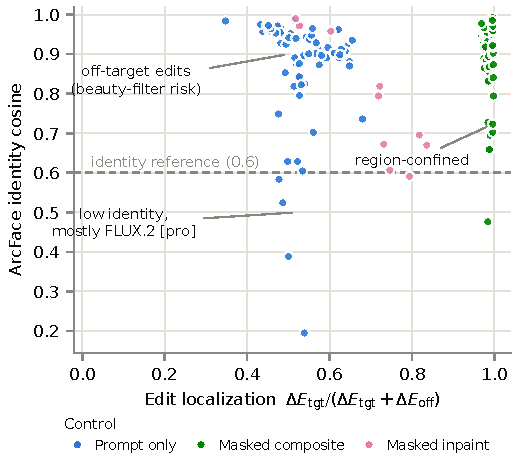
\includegraphics[width=\columnwidth]{scatter_identity_localization}
  \caption{Every scored edit, placed by the two failure modes. Masked compositing
  pins localization near 1 across models; prompt-only edits and the hosted
  inpainter leak roughly half their change off-target. All edits clear the
  identity floor.}
  \label{fig:scatter}
\end{figure}

Table~\ref{tab:main} and Fig.~\ref{fig:scatter} summarize the \NumScoredEdits{}
scored edits. We report medians and ranges throughout and make no statistical
significance claims at this sample size.

\subsection{Localization: the ladder works}

Masked compositing drives the localization ratio to a median of
\MedLocComposite{} (range \LocCompositeMin--\LocCompositeMax) regardless of which
model produced the edit. The same models under prompt-only control reach only
\MedLocPromptOnly{} (\LocPromptOnlyMin--\LocPromptOnlyMax): roughly half of the
measured change lands outside the surgical region, which is the beauty-filter
signature the metric was built to expose. The off-target numbers make the contrast
concrete---a median $\Delta E_{\mathrm{off}}$ of \MedOffPromptOnly{} for
prompt-only edits against \MedOffComposite{} for composited ones---while the
on-target change stays substantial (median $\Delta E_{\mathrm{tgt}}$
\MedTgtComposite{} composited vs.\ \MedTgtPromptOnly{} prompt-only). Prompt
guardrails alone, however carefully worded, did not confine the edit; moving the
confinement outside the model did.

\subsection{Identity}

Every scored edit clears the $0.6$ identity floor (minimum \IdentityMinAll{},
maximum \IdentityMaxAll). Following Sec.~\ref{sec:protocol}, the model-level
number is the prompt-only median of \MedIdentityPromptOnly{}: even without
compositing, current editors hold identity well above the floor on these faces.
Composited edits score a median of \MedIdentityComposite{}, but part of that is
copied pixels, so we do not read the difference as a model improvement.
Fig.~\ref{fig:boxes} breaks identity out by model; the ordering is consistent with
each model's editing aggressiveness rather than with output quality.

\begin{figure*}[t]
  \centering
  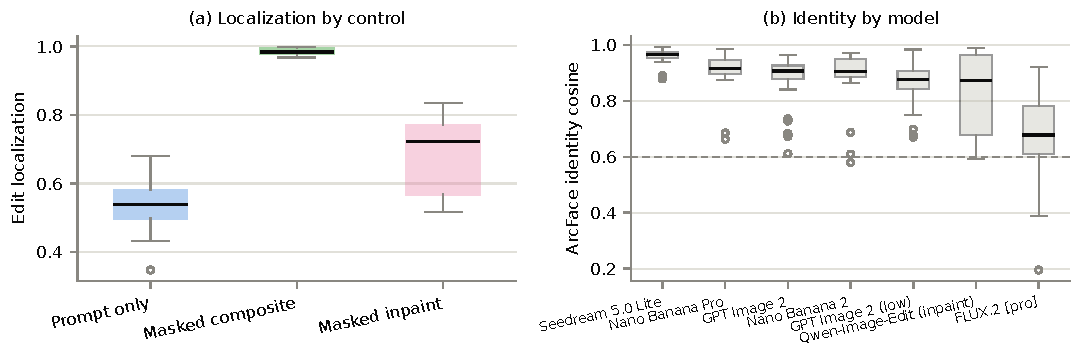
\includegraphics[width=0.92\textwidth]{box_localization_identity}
  \caption{(a) Localization by control rung, models pooled. (b) Identity by model,
  controls pooled; the dashed line is the acceptance floor. The hosted inpainter's
  near-perfect identity in (b) reflects under-editing, not superior preservation
  (see Sec.~\ref{sec:inpaint}).}
  \label{fig:boxes}
\end{figure*}

\subsection{Hosted inpainting under-edits}
\label{sec:inpaint}

The masked-inpaint rung was expected to dominate: the endpoint receives the mask
explicitly and should confine the edit for free. Instead it shows the protocol's
other failure mode. Its identity median of \MedIdentityInpaint{} is the highest in
the study, but its median target change is only \MedTgtInpaint{}---barely above
its off-target change of \MedOffInpaint{}, for a localization of just
\MedLocInpaint{} (\LocInpaintMin--\LocInpaintMax). The edit inside the mask is
timid, and the returned image differs slightly everywhere, consistent with a
full-image re-encode by the endpoint. Read jointly, the numbers say the hosted
inpainter mostly returned the input: exactly the deceptive near-copy the
did-nothing trap describes. At the tested endpoint, sending the mask to the model
was worse than ignoring the model's mask support entirely and compositing on the
client.

\subsection{Ground-truth sanity check}

Against real post-operative photographs the edits score a median cosine of
\MedGtCosine{} (range \GtCosineMin--\GtCosineMax; facelift
\MedGtCosineFacelift{}, rhinoplasty \MedGtCosineRhino), shown in
Fig.~\ref{fig:gt}. The values sit where same-person photographs taken months apart
under different pose, makeup, and hair typically land, which is all this check can
certify: the previews are not drifting toward a different person than the one the
surgery actually produced.

\begin{figure}[t]
  \centering
  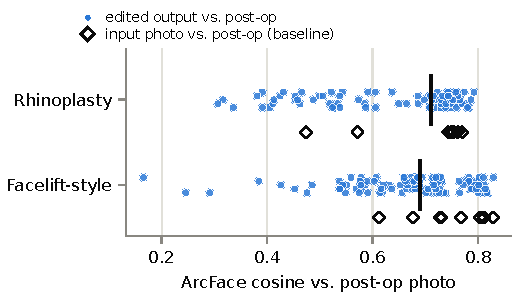
\includegraphics[width=\columnwidth]{strip_gt_cosine}
  \caption{ArcFace cosine between each edit and the face's real post-operative
  photograph (bars: medians). A soft sanity check; session differences cap the
  achievable score.}
  \label{fig:gt}
\end{figure}

\subsection{Chained procedures}

Chaining rhinoplasty and the facelift on the same face works in both orders:
identity \ChainedIdentityLow--\ChainedIdentityHigh{} and localization
\ChainedLocLow--\ChainedLocHigh{} for the two orderings ($n=\NumChained$), with no
visible interference between the nose and jaw--neck regions. Because the regions
are disjoint, each composited stage protects the other stage's canvas; order
appears to be a free parameter, though two probes on one face only establish
feasibility.

\subsection{Qualitative results and failure modes}

Fig.~\ref{fig:teaser} and Fig.~\ref{fig:grid} show representative edits. The
facelift examples display the intended tissue repositioning---jawline definition,
reduced jowls, a cleaner cervicomental angle---while skin texture, lighting, and
background survive untouched in the composited column. The characteristic failure
we observed before pose gating was the ghost seam: on profile views the
frontal-mesh mask landed on the cheek and composited a translucent copy of the
nose into it. Gating on yaw removed the artifact at the cost of leaving profile
inputs uncomposited, an honest gap that Sec.~\ref{sec:limitations} counts.

\begin{figure*}[t]
  \centering
  \includegraphics[width=0.88\textwidth]{qualitative_grid.png}
  \caption{Qualitative results (top to bottom: two deep-plane-facelift faces, one
  frontal rhinoplasty face). Prompt-only edits alter the whole image; composited
  edits are pixel-identical to the input outside the region.}
  \label{fig:grid}
\end{figure*}

\section{Limitations}
\label{sec:limitations}

This is a small pilot: \NumPrimaryFaces{} faces support the main comparisons,
each model--control cell has fewer than ten faces, and the chained probe uses one
additional face. Multiple outputs from one face are correlated; the clustered
interval addresses that dependence descriptively but cannot provide broad
population inference. Each cell contains one generated output, and two endpoints
ignore the supplied seed, so stochastic variation is unknown.

The localization ratio measures CIELAB pixel change, not anatomical direction,
clinical plausibility, realism, or expected postoperative appearance. Its keep
zone covers only part of the face and it abstains on profile views, precisely where
rhinoplasty visualization is important. Compositing guarantees off-mask
preservation, making that result a verification of system behavior rather than a
test of model quality. ArcFace's 0.6 line is heuristic, and the postoperative
cosines lack an input baseline; neither is a validated surgical-outcome metric.

No surgeon ratings were collected. Clinical plausibility therefore rests neither
on expert judgment nor on a clinically validated automated score. The demographic
composition of the face set was not recorded, so the results cannot be generalized
across skin tones, ages, or sexes; commercial face pipelines have documented
demographic disparities~\cite{buolamwini2018gendershades}. Public visibility of
the source photographs does not itself establish republication, hosted-processing,
or research-use permission, which must be resolved before submission.

Finally, hosted endpoints and aliases can change without notice. Run dates and
endpoint identifiers aid auditing but do not pin every underlying model revision.
The public repository contains the canonical score table and paper analysis, not
the complete generation/scoring implementation or source photographs, so the
study is not presently reproducible end to end.

\section{Ethics and Privacy}
% Data provenance (synthetic + publicly available before/after photos; no private
% patient data); licensing/attribution; no cherry-picking; previews as expectation
% aids, not guarantees; misuse; demographic-fairness gap.
\todo{ethics and privacy}

\section{Conclusion}
\label{sec:conclusion}

In this pilot, text instructions alone did not prevent image-editing APIs
from changing a predefined facial keep zone. A landmark-derived mask,
alignment, and client-side feathered composite reduced that measured off-target
change while retaining similar target-region pixel change, uniformly across the
six editors tested and at a median provider cost of \$\MedCost{} per image. The
tested Qwen inpainting model did not outperform that post-hoc control, but
one model cannot support a general conclusion about masked inpainting.

The study does not validate cosmetic-surgery outcome prediction, and
client-side compositing should be read as a control for off-target pixel
changes, not as evidence that a preview is clinically accurate or safe for
patient counseling. The main analysis contains \NumPrimaryFaces{} faces, one
generated output per cell, no surgeon ratings, limited profile support, and
only an identity-embedding measure of movement toward the postoperative
photographs; by that measure the edits moved slightly away from the outcome,
not closer. The next study should add repeated generations, pose-robust
whole-image localization, and anatomy-aware postoperative accuracy metrics. It will
also need multiple blinded surgeons with inter-rater agreement, a larger and
demographically characterized cohort, and immutable or self-hosted model
baselines. What the pilot does establish is
narrower: when an editor exposes no internals, region confinement can still be
enforced entirely from the client.


\nocite{*} % TODO: remove once sections cite explicitly (Session 4)
\bibliographystyle{IEEEtran}
\bibliography{refs}

\end{document}
